\begin{frame}{Learning objectives}
\begin{itemize}
\item Fit and interpret a simple OLS regression.
\item Connect residuals, $R^2$, standard errors and intervals.
\item Use multiple predictors, dummy variables and interactions.
\item Diagnose unusual observations and model misspecification.
\item Evaluate predictions on observations not used to fit the model.
\end{itemize}
\end{frame}

\begin{frame}{Conditional means and individual outcomes}
\[Y_i=\beta_0+\beta_1X_i+\varepsilon_i,\qquad E(\varepsilon_i\mid X_i)=0.\]\begin{itemize}
\item $\beta_0+\beta_1X_i$ is the conditional mean.
\item $\varepsilon_i$ is the individual deviation from that mean.
\item The slope expresses an association in the specified model.
\item The fitted line estimates the unknown population relationship.
\end{itemize}
\end{frame}

\begin{frame}{A small worked example}
\begin{center}\begin{tabular}{lrrrrr}\toprule
Student & A & B & C & D & E\\\midrule Study hours $x$ & 2 & 3 & 4 & 5 & 6\\ Score $y$ & 50 & 55 & 60 & 63 & 72\\
\bottomrule\end{tabular}\end{center}Five fictional observations, used to make the arithmetic transparent.\prompt{Sketch a line through these points. What would a slope of 5 mean?}
\end{frame}

\begin{frame}{Fitted values and residuals}
\[\hat y_i=\hat\beta_0+\hat\beta_1x_i,\qquad e_i=y_i-\hat y_i.\]\begin{itemize}
\item A residual is positive when the observed value lies above the fitted line.
\item Residuals are calculated from the fitted model; errors are unobserved population quantities.
\item OLS chooses the coefficients that minimise $\mathrm{SSE}=\sum_i e_i^2$.
\end{itemize}
\end{frame}

\begin{frame}{The least-squares estimates}
\[\hat\beta_1=\frac{\sum_i(x_i-\bar x)(y_i-\bar y)}{\sum_i(x_i-\bar x)^2},\qquad\hat\beta_0=\bar y-\hat\beta_1\bar x.\]\begin{itemize}
\item The predictor must vary: the denominator must be positive.
\item Using the same covariance and variance convention, $\hat\beta_1=s_{xy}/s_x^2$.
\item The fitted line passes through $(\bar x,\bar y)$.
\end{itemize}
\end{frame}

\begin{frame}{Calculating the line}
\[\bar x=4,\quad\bar y=60,\quad S_{xx}=10,\quad S_{xy}=52.\]\[\hat\beta_1=52/10=5.2,\qquad\hat\beta_0=60-5.2(4)=39.2.\]\[\boxed{\hat y=39.2+5.2x}\]One additional study hour is associated with a 5.2-point difference in predicted score.
\end{frame}

\begin{frame}{Reading the intercept}
\begin{itemize}
\item The intercept predicts the outcome at $x=0$.
\item Our observations cover 2--6 hours; zero lies outside that range.
\item An intercept may be algebraically necessary without a useful substantive interpretation.
\item Centring $x$ at 4 hours gives $\hat y=60+5.2(x-4)$, with a meaningful reference value.
\end{itemize}
\end{frame}

\begin{frame}{Residuals in the example}
\begin{center}\begin{tabular}{rrrr}\toprule
$x$ & $y$ & $\hat y$ & $e$\\\midrule 2 & 50 & 49.6 & 0.4\\3 & 55 & 54.8 & 0.2\\4 & 60 & 60.0 & 0.0\\5 & 63 & 65.2 & -2.2\\6 & 72 & 70.4 & 1.6\\
\bottomrule\end{tabular}\end{center}\[\sum_i e_i=0,\qquad \mathrm{SSE}=7.60.\]
\end{frame}

\begin{frame}{Visualising residuals}
\centering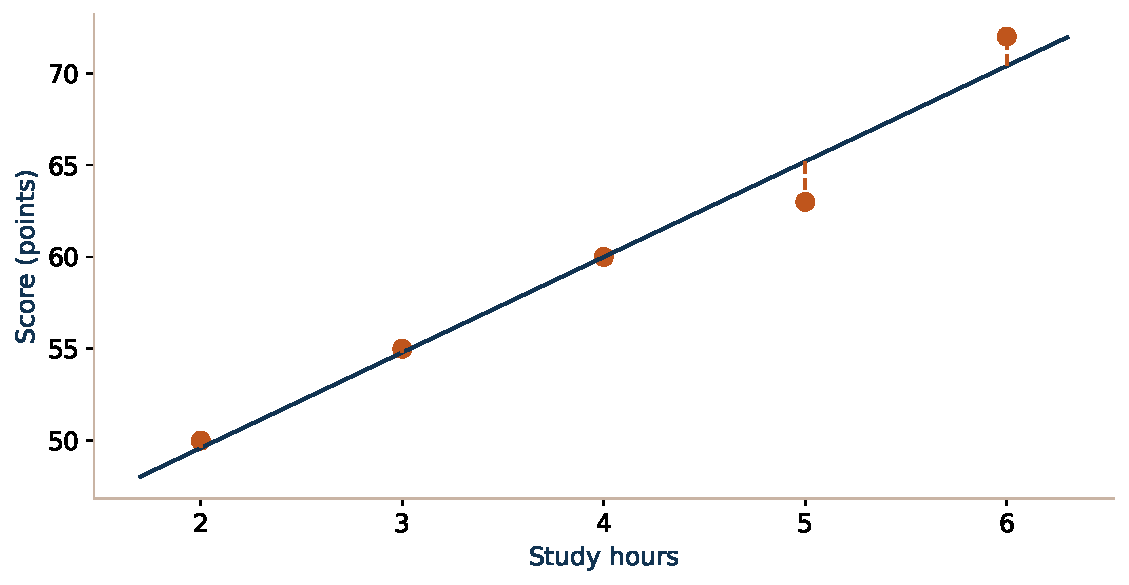
\includegraphics[width=.86\textwidth,height=.64\textheight,keepaspectratio]{figures/supervised/ols_residuals.pdf}
\end{frame}

\begin{frame}{Decomposition of variation}
For OLS with an intercept,\[\underbrace{\sum_i(y_i-\bar y)^2}_{\mathrm{SST}}=\underbrace{\sum_i(\hat y_i-\bar y)^2}_{\mathrm{SSR}}+\underbrace{\sum_i(y_i-\hat y_i)^2}_{\mathrm{SSE}}.\]\begin{itemize}
\item SST: total observed variation around the sample mean.
\item SSR: variation represented by the fitted values.
\item SSE: variation remaining in residuals.
\end{itemize}
\end{frame}

\begin{frame}{R-squared}
\[R^2=1-\frac{\mathrm{SSE}}{\mathrm{SST}}=1-\frac{7.6}{278}=0.9727.\]\begin{itemize}
\item About 97.3\% of the sample variation is represented by this fitted line.
\item This is an in-sample measure, not a causal explanation.
\item In simple OLS with an intercept, $R^2=r_{xy}^2$.
\item High $R^2$ does not establish model validity or good future predictions.
\end{itemize}
\end{frame}

\begin{frame}{Residual standard error}
\[s=\sqrt{\frac{\mathrm{SSE}}{n-2}}=\sqrt{\frac{7.6}{3}}=1.592.\]\begin{itemize}
\item Measured in the same units as the outcome: score points.
\item The denominator accounts for two estimated coefficients.
\item With $p$ predictors and an intercept, the full-rank model uses $n-p-1$ residual degrees of freedom.
\end{itemize}
\end{frame}

\begin{frame}{Assumptions and what they support}
\begin{itemize}
\item OLS minimisation is algebra; it does not require Normality.
\item A correct conditional-mean specification and zero conditional-mean errors support coefficient interpretation and unbiasedness under fixed full-rank design.
\item Independence and appropriate sampling connect the model with a target population.
\item Constant conditional variance supports the usual OLS standard errors.
\item Independent Normal errors with common variance give exact finite-sample $t$ and $F$ inference.
\end{itemize}
\end{frame}

\begin{frame}{Standard error and slope interval}
Under the classical simple-regression model,\[\mathrm{SE}(\hat\beta_1)=\frac{s}{\sqrt{S_{xx}}}=0.5033.\]\[\hat\beta_1\pm t_{n-2,.975}\,\mathrm{SE}(\hat\beta_1)=5.2\pm3.182(0.5033)=[3.598,6.802].\]This 95\% interval concerns the population slope. Its coverage statement is about repeated sampling under the model.
\end{frame}

\begin{frame}{Testing the slope}
\[H_0:\beta_1=0,\qquad H_1:\beta_1\ne0.\]\[t=\frac{5.2}{0.5033}=10.331,\quad df=3,\quad p=0.00193.\]\begin{itemize}
\item The p-value assesses compatibility with the null under the assumptions.
\item It is not the probability that the null is true.
\item A small p-value does not establish causality or practical usefulness.
\end{itemize}
\end{frame}

\begin{frame}{The regression ANOVA connection}
\[F=\frac{\mathrm{SSR}/1}{\mathrm{SSE}/(n-2)}=t^2=106.737.\]\begin{itemize}
\item In simple regression, the global $F$ test and the two-sided slope $t$ test have the same p-value.
\item This equality uses the classical OLS variance estimator.
\item With several predictors, the global $F$ test asks whether all tested slopes are zero; it is not one individual $t$ test.
\end{itemize}
\end{frame}

\begin{frame}{Mean confidence interval or prediction interval?}
\centering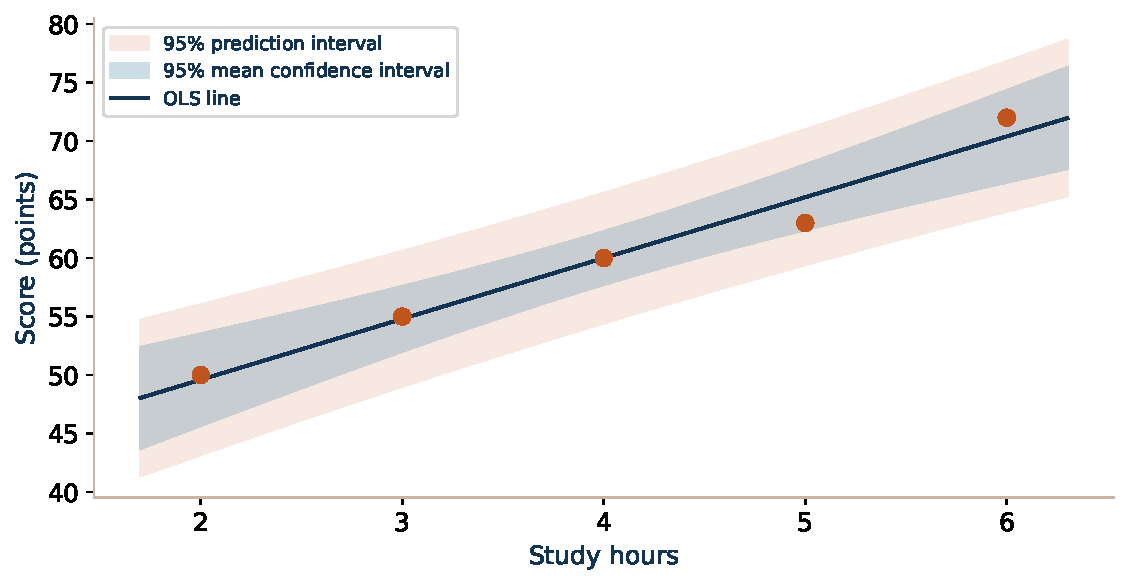
\includegraphics[width=.86\textwidth,height=.64\textheight,keepaspectratio]{figures/supervised/linear_intervals.pdf}\par\small The prediction interval includes individual outcome variation and is wider. Both rely on the model assumptions.
\end{frame}

\begin{frame}{Prediction and extrapolation}
\begin{itemize}
\item At 5 hours: $\hat y=65.2$ points.
\item At 8 hours: $\hat y=80.8$ points, outside the observed 2--6 hour range.
\item The relation may change outside the observed range.
\item A mathematical prediction does not ensure plausibility: an unbounded linear model can predict scores above the scale maximum.
\end{itemize}
\end{frame}

\begin{frame}{Multiple linear regression}
\[E(Y\mid\mathbf X)=\beta_0+\beta_1X_1+\cdots+\beta_pX_p.\]\begin{itemize}
\item A slope describes a conditional association, holding the other included predictors fixed.
\item Adding a predictor can change the coefficient of an existing predictor.
\item Correlated predictors can make individual coefficients imprecise.
\item The design matrix must have full column rank for a unique coefficient vector.
\end{itemize}
\end{frame}

\begin{frame}{A fictional housing example}
\[\text{price}=\beta_0+\beta_1\text{area}+\beta_2\text{renovated}+\beta_3\text{centre}+\varepsilon.\]\begin{itemize}
\item Price is measured in thousands of euros; area is in square metres.
\item Renovated and centre are binary predictors defined before the prediction.
\item Interpret $\beta_1$ as a price difference per square metre, conditional on the other included predictors.
\item These simulated data do not describe any real housing market.
\end{itemize}
\end{frame}

\begin{frame}{Categorical predictors and reference categories}
\begin{itemize}
\item For a binary variable $D$, use 0 for the reference group and 1 for the comparison group.
\item In $E(Y)=\beta_0+\beta_1x+\beta_2D$, $\beta_2$ shifts the intercept.
\item For $k$ categories, use $k-1$ indicators when including an intercept.
\item Coding categories as 1, 2, 3 imposes a quantitative spacing that may not be meaningful.
\end{itemize}
\end{frame}

\begin{frame}{Interactions}
\[E(Y\mid x,D)=\beta_0+\beta_1x+\beta_2D+\beta_3xD.\]\begin{center}\begin{tabular}{ll}\toprule
$D=0$ & $\beta_0+\beta_1x$\\ $D=1$ & $(\beta_0+\beta_2)+(\beta_1+\beta_3)x$\\ Group difference at $x$ & $\beta_2+\beta_3x$\\
\bottomrule\end{tabular}\end{center}The main effect of $D$ is now the difference at $x=0$. Centring $x$ can make that reference more useful.
\end{frame}

\begin{frame}{Parallel lines and interactions}
\centering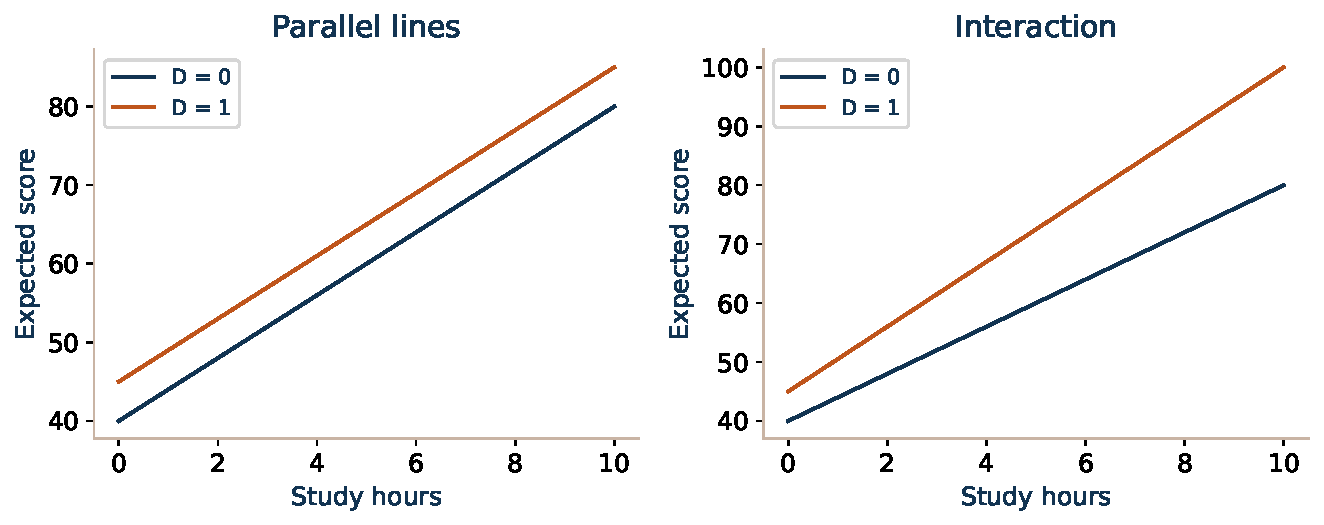
\includegraphics[width=.86\textwidth,height=.64\textheight,keepaspectratio]{figures/supervised/dummy_interaction.pdf}
\end{frame}

\begin{frame}{A worked interaction}
Consider the illustrative model\[\hat y=40+4x+5D+1.5xD.\]\begin{itemize}
\item At $D=0$: slope $=4$, intercept $=40$.
\item At $D=1$: slope $=5.5$, intercept $=45$.
\item At $x=4$: predictions are 56 and 67; the group difference is 11.
\end{itemize}A nonsignificant interaction is not proof that the two slopes are identical.
\end{frame}

\begin{frame}{Nonlinearity in predictors}
\[E(Y\mid x)=\beta_0+\beta_1x+\beta_2x^2.\]\begin{itemize}
\item This model is linear in the coefficients, but curved in $x$.
\item The local slope is $\beta_1+2\beta_2x$.
\item Higher polynomial degree adds flexibility and can increase overfitting.
\item Assess predictive complexity using validation or cross-validation.
\end{itemize}
\end{frame}

\begin{frame}{Residual diagnostics}
\centering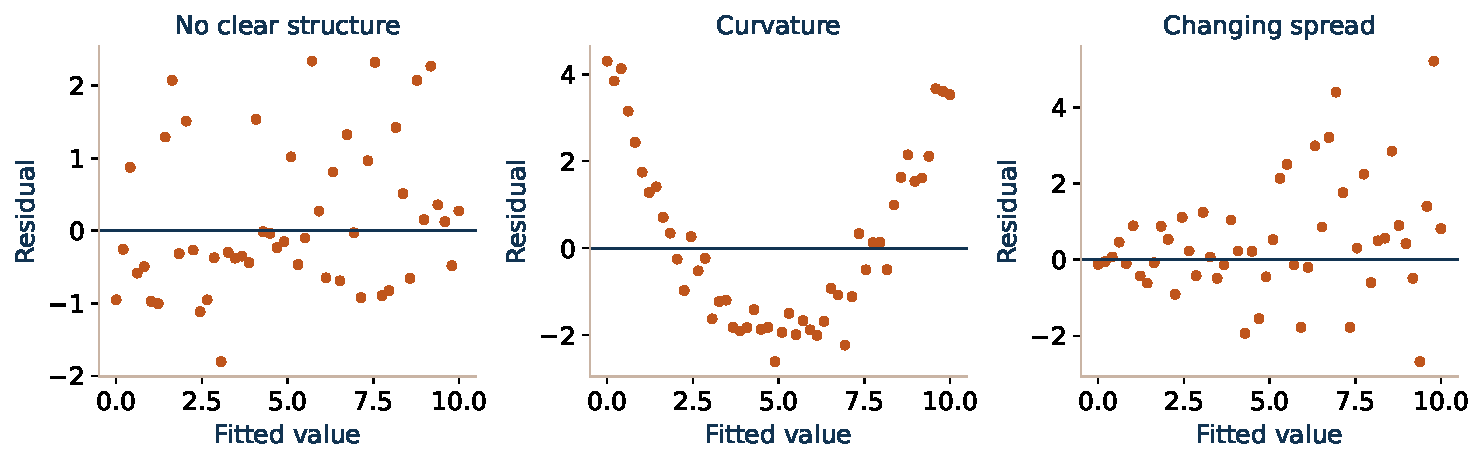
\includegraphics[width=.86\textwidth,height=.64\textheight,keepaspectratio]{figures/supervised/residual_patterns.pdf}\par\small Illustrative patterns. A residual plot can reveal a problem; a pattern-free plot does not prove every assumption.
\end{frame}

\begin{frame}{Outliers, leverage and influence}
\begin{center}\begin{tabular}{lp{.62\textwidth}}\toprule
Concept & Diagnostic question\\\midrule Unusual residual & Is $y$ far from its fitted value?\\ High leverage & Is the predictor combination unusual?\\ Influence & Does this observation substantially change the fitted model?\\
\bottomrule\end{tabular}\end{center}Cook\textquotesingle s distance combines residual size and leverage. A high-leverage point need not be influential.
\end{frame}

\begin{frame}{Investigating an unusual observation}
\begin{itemize}
\item Check measurement, coding and population membership.
\item Inspect the point in context, not just against a numerical threshold.
\item Compare estimates with and without it as a sensitivity analysis.
\item Report the effect of any exclusion and justify the decision.
\item Do not remove valid observations simply to improve significance or $R^2$.
\end{itemize}
\end{frame}

\begin{frame}{Heteroskedasticity and robust standard errors}
\begin{itemize}
\item Unequal conditional error variances can invalidate classical standard errors.
\item Heteroskedasticity-consistent standard errors change estimated uncertainty, not OLS coefficients.
\item They do not fix omitted-variable bias, nonlinearity or dependence.
\item HC3 is implemented in the R lab; the reported robust intervals use a large-sample Normal approximation.
\end{itemize}
\end{frame}

\begin{frame}{Log transformations}
\begin{center}\begin{tabular}{lp{.58\textwidth}}\toprule
Model & Interpretation of $\beta_1$\\\midrule $\log Y=\beta_0+\beta_1x+\varepsilon$ & A one-unit increase in $x$ multiplies the fitted geometric mean by $e^{\beta_1}$.\\ $Y=\beta_0+\beta_1\log x+\varepsilon$ & A 1\% increase in $x$ changes the fitted mean by approximately $\beta_1/100$ units.\\ $\log Y=\beta_0+\beta_1\log x+\varepsilon$ & A 1\% increase in $x$ changes the fitted geometric mean by approximately $\beta_1$\%.\\
\bottomrule\end{tabular}\end{center}Natural logs require positive values. Check which variable is transformed.
\end{frame}

\begin{frame}{Exact percentages and retransformation}
\begin{itemize}
\item In a log-response model, a coefficient of 0.10 corresponds to $100(e^{0.10}-1)=10.52\%$ on the fitted geometric-mean scale.
\item Exponentiating a predicted log outcome does not generally give $E(Y\mid X)$.
\item Under suitable error assumptions, a lognormal correction or a smearing estimate can target an arithmetic mean.
\item The R lab estimates the smearing factor from training residuals only.
\end{itemize}
\end{frame}

\begin{frame}{Prediction metrics on new data}
\[\mathrm{RMSE}=\sqrt{\frac1m\sum_{i=1}^m(y_i-\hat y_i)^2},\qquad\mathrm{MAE}=\frac1m\sum_{i=1}^m|y_i-\hat y_i|.\]\begin{itemize}
\item Use predictions for observations excluded from fitting and selection.
\item Compare with a mean or median baseline learned from training data.
\item A test-set $R^2$ can be negative when predictions are worse than the test-mean benchmark.
\end{itemize}
\end{frame}

\begin{frame}{More predictors do not guarantee better predictions}
\begin{itemize}
\item Training SSE cannot increase when adding predictors to nested OLS models.
\item Training $R^2$ therefore cannot decrease.
\item Adjusted $R^2$ penalises model size, but is still based on the fitted sample.
\item Use cross-validation for predictive selection; retain the test set for final evaluation.
\item Inference after data-driven model selection requires additional care.
\end{itemize}
\end{frame}

\begin{frame}{R laboratory}
\begin{itemize}
\item \texttt{01\_ols\_by\_hand.R}: coefficients, residuals, tests and intervals.
\item \texttt{02\_multiple\_diagnostics.R}: indicators, interactions, HC3 and logs.
\item \texttt{04\_validation\_and\_cv.R}: model selection and final prediction metrics.
\item Read outputs in context; a numerical result needs an interpretation and a stated limitation.
\end{itemize}
\end{frame}

\begin{frame}{Applied task}
\prompt{Using the housing data, compare an area-only model with an additive model and a model with an area-by-centre interaction.}\begin{itemize}
\item State the target and units.
\item Interpret a coefficient and a conditional group difference.
\item Inspect residuals and influential cases.
\item Use the supplied split or development-set cross-validation.
\item Report final predictive performance without retuning on the test set.
\end{itemize}
\end{frame}

\begin{frame}{Checkpoint}
\begin{itemize}
\item What does OLS minimise? Why square the residuals?
\item What changes when we add a dummy and an interaction?
\item How does a confidence interval differ from a prediction interval?
\item Why is a high $R^2$ insufficient?
\item What does a robust standard error fix, and what does it leave unresolved?
\end{itemize}
\end{frame}

\begin{frame}{Appendix: normal equations}
\[Q(b_0,b_1)=\sum_i(y_i-b_0-b_1x_i)^2.\]\[\frac{\partial Q}{\partial b_0}=-2\sum_i(y_i-b_0-b_1x_i)=0,\]\[\frac{\partial Q}{\partial b_1}=-2\sum_ix_i(y_i-b_0-b_1x_i)=0.\]The first equation gives $b_0=\bar y-b_1\bar x$. Substitution into the second gives the OLS slope formula.
\end{frame}

\begin{frame}{Appendix: interval formulas}
For a simple classical regression, let $\hat y_0=\hat\beta_0+\hat\beta_1x_0$.\[\text{Mean CI: }\quad \hat y_0\pm t_{n-2,1-\alpha/2}s\sqrt{\frac1n+\frac{(x_0-\bar x)^2}{S_{xx}}}.\]\[\text{Individual PI: }\quad \hat y_0\pm t_{n-2,1-\alpha/2}s\sqrt{1+\frac1n+\frac{(x_0-\bar x)^2}{S_{xx}}}.\]The extra 1 represents the variance of a new independent error. Both intervals widen away from $\bar x$.
\end{frame}
